\documentclass[	11pt,		% 11 Punkte hohe Schrift
				a4paper,	% Einstellung des Ausdrucks auf DIN A4
				fleqn,		% linksbündige, abgesetzte Formeln
				reqno,		% rechts stehende Formelnummer
				BCOR12mm,	% Bindekorrektur von 12mm
				chapterprefix=false,	% Ausgabe von Kapitel: 
				appendixprefix=true, % Überschrift im Anhang X und dann neue Zeile und Titel
				parskip=half,
				DIV=calc,
				final,		% Abgabe Version
]{scrartcl}
%\usepackage{natbib}
\usepackage{packages}
\usepackage{layout}
\usepackage{hyperref}
\graphicspath{{image/}}
\DeclareGraphicsExtensions{.png,.pdf}

\bibliography{src/literatur}	% Literaturverzeichnis

\newtheorem{defi}{Definition}
\newtheorem{bsp}{Beispiel}
\newtheorem{satz}{Satz}
\newtheorem{theo}{Theorem}

\newcommand{\bspautorefname}{Beispiel}
\newcommand{\defiautorefname}[1]{Definition #1}
\newcommand{\theoautorefname}{Theorem}

\newcommand{\RM}[1]{\MakeUppercase{\romannumeral #1{}}} 

\begin{document}
	% Cover
	\begin{titlepage}
  \begin{centering}
  \begin{figure}[h!]
    \centering
    
\includegraphics[width=310pt]{UniLogo}
  \end{figure}

  \vspace*{-0.8cm}

  \begin{figure}[h!]
    \centering
    
\includegraphics[width=280pt]{BUIENGLOGO}
  \end{figure}

  \vspace*{0.4cm}
  
  \textsf{\Huge \textbf{Projektgruppe FAISE\\}}

  \vspace*{0.5cm}
  \noindent Endbericht\\
  im Rahmen des Masterstudiums

  \end{centering}
  
  \vspace*{1.5cm}
  \begin{tabbing}
  xxxxxxxxxxxxxxxx\= \kill
  
  \small Betreuer: \>Prof. Dr.-Ing. Jürgen Sauer\\
  \small \>Dipl.-Ing. (FH) Arne Stasch\\
  \small \>Dipl.-Inform. Jan-Hinrich Kämper\\
  \small \>Prof. Dr.-Ing. Axel Hahn\\\\

  \small Vorgelegt von: \>Berthe Pulcherie Ongnomo\\
  \small \>Chancelle Merveille Tematio Yme\\
  \small \>Christopher Schwarz\\
  \small \>Jan Paul Vox\\
  \small \>Jan-Gerd Meß\\
  \small \>Jannik Fleßner\\
  \small \>Malte Falk\\
  \small \>Mathias Aden\\
  \small \>Michael Goldenstein\\
  \small \>Nagihan Aydin\\
  \small \>Raschid Alkhatib\\
  \small \>Simon Jakubowski\\\\

  \small Abgabetermin:\> 30. September 2014
  \end{tabbing}
\end{titlepage}
	\pagenumbering{Roman}
	% Abstract
	\include{src/abstract}

	% Table of contents
	\clearpage
\ohead[Inhaltsverzeichnis]{Inhaltsverzeichnis}
\chead[Uni Oldenburg]{Uni Oldenburg}
\ihead[PG FAISE]{PG FAISE}
\setheadtopline{1pt}
\setheadsepline{0.5pt}

\ofoot[Endbericht]{Endbericht}
\cfoot[\pagemark]{\pagemark}
\ifoot[30. September 2014]{30. September 2014}
\setfootsepline{0.5pt}
\setfootbotline{1pt}

\tableofcontents
\clearpage

\ohead[Abbildungsverzeichnis]{Abbildungsverzeichnis}
\chead[Uni Oldenburg]{Uni Oldenburg}
\ihead[PG FAISE]{PG FAISE}
\setheadtopline{1pt}
\setheadsepline{0.5pt}

\ofoot[Endbericht]{Endbericht}
\cfoot[\pagemark]{\pagemark}
\ifoot[30. September 2014]{30. September 2014}
\setfootsepline{0.5pt}
\setfootbotline{1pt}

\listoffigures
%\listoftables
	
	% Chapter 1 Einleitung
	\pagenumbering{arabic}
	\clearpage
	\ohead[Einleitung]{Einleitung}
	\chead[Uni Oldenburg]{Uni Oldenburg}
	\ihead[PG FAISE]{PG FAISE}
	\setheadtopline{1pt}
	\setheadsepline{0.5pt}
	\ofoot[Endbericht]{Endbericht}
	\cfoot[\pagemark]{\pagemark}
	\ifoot[30. September 2014]{30. September 2014}
	\setfootsepline{0.5pt}
	\setfootbotline{1pt}
	\section{Einleitung}
In diesem Kapitel wird ein einführender Überblick über die Projektgruppe Fully Autonomous Intralogistic Swarm Experiments gegeben, die im Rahmen der Masterstudiengänge Informatik und Wirtschaftsinformatik in der Abteilung Systemanalyse und -optimierung der Carl von Ossietzky Universität Oldenburg stattgefunden hat. Das Projekt lief über einen Zeitraum von zwei Semestern: Wintersemester 2013/2014 und Sommersemester 2014.


\subsection{Motivation}
Im Zeitalter der Globalisierung werden hohe Anforderungen an die Leistungsfähigkeit von modernen Intralogistiksystemen gestellt. Neben einem hohen Automatisierungsgrad wird gleichzeitig auch eine möglichst hohe Flexibilität gefordert, da sich Anforderungen im logistischen Umfeld häufig ändern (Vgl.\cite{ieft}).    
\\\\
Stetigförderer bieten die Möglichkeit einen automatisierten Materialfluss einzurichten. Es handelt sich dabei um Transportsysteme, die Güter kontinuierlich und automatisiert entlang eines festgelegten Transportwegs befördern (Vgl.\cite{stf}). Ein solches System könnte beispielsweise ein Netz von Schienen sein. Nachteile dieser Systeme sind insbesondere Unflexibilität und schlechte Skalierbarkeit. Ändern sich Anforderungen in einem Logistiksystem, dann stoßen Stetigförderer schnell an ihre Grenzen. Transportwege sind festgelegt und können nicht ohne einen gewissen Aufwand geändert werden. Auch kann die Anzahl an Gütern, die pro Zeiteinheit befördert werden kann, nicht ohne eine Änderung am Transportnetz maximiert werden.
\\\\
Eine Alternative zu Stetigförderern sind Fahrerlose Transportsysteme (FTS). FTS sind ein Gesamtsystem aus Fahrerlosen Transportfahrzeugen, die Ware automatisiert befördern, und der Infrastruktur, die zum Betrieb der Transporteinheiten notwendig ist (Vgl.\cite{fts}). Fahrerlose Transportsysteme sind wesentlich flexibler als Stetigförderer. Müssen mehr Güter befördert werden, so können zusätzliche Transporteinheiten aktiviert werden. Folglich sind FTS problemlos skalierbar und können schnell auf veränderte Anforderungen in einem Intralogistiksystem eingestellt werden. FTS bieten einen automatisierten Warenfluss bei gleichzeitig hoher Flexibilität und entsprechen somit den Anforderungen, die an moderne Intralogistiksysteme gestellt werden.  
\\\\
%Es bietet sich an ein System zu entwickeln, das basierend auf FTS, einen vollautomatisierten %Warenfluss implementiert, um verschiedene Fragestellungen zu untersuchen. Wie muss ein solches %System aufgebaut sein, welche Kommunikationsabläufe sind zwischen den verschiedenen Akteuren %notwendig, welche Anforderungen werden an Hard- und Software gestellt und wie flexibel ist ein %solches System?  

\subsection{Zielsetzung}
Im Rahmen der Projektgruppe FAISE soll ein System entwickelt werden, das den vollautomatisierten Warenfluss in einem Lager auf Basis von Fahrerlosen Transportsystemen simuliert. Dabei sollen die Transporteinheiten nicht zentral gesteuert werden, sondern dezentral agieren.
Das Gesamtsystem besteht aus zwei Teilsystemen, einem physisch vorhandenem System und einer softwarebasierten Simulation. 
\\\\
Das physische System beinhaltet Rampen, auf denen Ware gelagert werden kann und Fahrerlose Transporteinheiten als Fördermittel. Die Akteure kommunizieren miteinander über ein Sensornetzwerk und werden auf Basis von Mikrocontrollern gesteuert. Ziel ist es den Materialfluss von den Transporteinheiten und Rampen vollständig autonom und ohne dezentrale Steuerung durchzuführen. 
\\\\
Das rein softwarebasierte System soll einen automatisierten Warenfluss, der durch Rampen und Fahrzeuge durchgeführt wird, simulieren. Die Realisierung der Akteure in der Software soll an die Eigenschaften der Akteure aus dem physische System angelehnt sein. Beide Systeme sollen unabhängig voneinander laufen. 

\subsection{Einsatzszenario}\label{Einsatzszenario} 
Das Einsatzszenario besteht aus n fahrerlosen Transporteinheiten in einem Umschlagslager. Zusätzlich sind m Rampen verfügbar an denen Pakete zwischengelagert werden können. Im Gegensatz zu einem herkömmlichen Lager, werden Waren in einem Umschlagslager nur kurzfristig gelagert, um anschließend weitertransportiert zu werden. Es herrscht ein kontinuierlicher Materialfluss. Jedes Paket, das ins Lager gebracht wird, ist eindeutig identifizierbar und wird zu einem definierten Zeitpunkt ins Lager gebracht und wieder abgeholt. Die Rampen im Lager sollen drei unterschiedliche Zwecke erfüllen. Eingangsrampen dienen der Warenannahme, Zwischenrampen der Zwischenlagerung. Pakete werden zum Ausgangslager gebracht und zum Zwecke des Weitertransports dort abgeholt. Auf Basis des Einsatzszenarios wird im Rahmen der Anforderungen ein Ablaufszenario erstellt, das die Interaktionen zwischen den Akteuren beschreibt auf deren Basis eine automatisierte, dezentrale Abwicklung des Materialflusses erfolgen kann.

\subsection{Komponenten}
Das zu entwickelnde System lässt sich grob in die Komponenten physisches System und Simulation unterteilen. Das physisches System wiederum lässt sich noch weiter in die Komponenten Materialfluss und Fahrzeuge aufteilen. Das Gesamtsystem lässt sich somit in drei Komponente aufteilen, die im Folgenden beschrieben werden:

\begin{itemize}
\item Materialfluss: Die Komponente Materialfluss beschreibt die Rampen auf denen Pakete gelagert werden. Die Rampen sollen mithilfe von Sensoren mit anderen Rampen und den fahrerlosen Transporteinheiten kommunizieren können. Durch Aktoren soll es möglich sein, Pakete zum Zwecke des Weitertransports an die Fahrzeuge zu übergeben.
\item Fahrzeuge: Die Fahrzeuge übernehmen den Transport der Pakete und kommunizieren mit den Rampen, um den Transport automatisiert abzuwickeln. Die Fahrzeuge sollen anhand von Start- und Zielpunkten in der Lage sein, selbstständig Pfade zu erstellen und diese abzufahren.
\item Simulation: Die Simulation soll als Softwaresystem realisiert werden, dass es erlaubt Szenarien mit einer bestimmten Anzahl an Rampen und Fahrzeugen zu erstellen. Wie im physischen System, sollen die Rampen und Fahrzeuge einen automatisierten Warenfluss durchführen und die Aktionen sollen visualisiert werden.  
\end{itemize} 

	
	% Chapter 2 Stand der Technik
	\clearpage
	\ohead[Stand der Technik]{Stand der Technik}
	\chead[Uni Oldenburg]{Uni Oldenburg}
	\ihead[PG FAISE]{PG FAISE}
	\setheadtopline{1pt}
	\setheadsepline{0.5pt}
	\ofoot[Endbericht]{Endbericht}
	\cfoot[\pagemark]{\pagemark}
	\ifoot[30. September 2014]{30. September 2014}
	\setfootsepline{0.5pt}
	\setfootbotline{1pt}
	\section{Stand der Technik}
Die Fahrerlosen Transportsysteme und die Materialflusssysteme sind Prozesse der Logistik. In den vergangenen Jahren hat die Verbreitung Fahrerloser Transportsysteme (FTS) stark zugenommen. Beim Einsatz von FTS stellen sich vielfältige Konfigurierungs- und Planungsprobleme, so auch die Einsatzplanung f\"ur die einzelnen Fahrerlosen Transportfahrzeuge. (vgl. Günther; Krüger; Schrecker; 2000, S. 2). Der innerbetriebliche Materialfluss von Industrieunternehmen bietet fahrerlosen Transportsystemen (FTS) zahlreiche Einsatzgebiete: Sie verketten Produktionsprozesse, verknüpfen Fertigungsstationen oder ganze Betriebsbereiche und beschicken Montageplätze. Darüber hinaus dienen sie als mobile Werkbank oder versorgen und entsorgen Lager unterschiedlicher Art. Um die Systemvorteile von Fahrerlosen Transportsystemen und Materialflusssystemen zu optimieren, braucht man ein ma\ss gerechtes Wissen auf Ihr spezifisches Anlagekonzept abzustimmen. Wichtige Kriterien sind allerdings z.~B. die Einbindung der Fahrerlosen Transportsysteme in den gesamtbetrieblichen Materialfluss, die Anpassung an die vorhandenen Steuerungshierarchien und die optimale Auslegung der Technik in Bezug auf Fahrzeugbauart, Lastaufnahmemittel, Energiekonzept, Kommunikation und Leitsystem. (vgl. Werner Swoboda, Industrie Anzeiger). Ziele von Fahrerlosen Transportsystemen und Materialflusssystemen sind Kostensenkung durch Personaleinsparung, Verringerung von Transportsch\"aden, hohe Zuverl\"assigkeit in Vorg\"angen und bessere Materialflussplanung.
Dieses Kapitel wird in drei Teile gegliedert. Der erste Teil wird die Fahrerlosen Transportsysteme bzw die Orientierungs- und die Steuerungssysteme vorstellen und erkl\"aren; der zweite Teil ist eine Darstellung der Materialflusssysteme und ihrer verschiedenen Funktionen und der dritte Teil wird erkl\"aren, wie fahrerlose Transport- und Materialflusssysteme in gro\ss en Firmen wie Volkswagen und BMW Anwendung finden.

\subsection{Fahrerlose Transportsysteme}
Nach dem Verein Deutscher Ingenieure 2510 bestehen FTS im Wesentlichen aus "`einem oder mehreren Fahrerlosen Transportfahrzeugen (FTF), einer Leitsteuerung, Einrichtung zur Standortbestimmung und Lagererfassung, Einrichtungen zur Daten\"ubertragung sowie Infrastruktur und peripheren Einrichtungen"'. In seinem Buch Transport und Lagerlogistik fasst Martin die Definition von VDI 2510 eines FTS zusammen. Er beschreibt ein FTS als mit FTF ausgestattete rechnergesteuerte Materialflussanlagen zum automatischen Transport von G\"utern im innerbetrieblichen Materialfluss. (vgl. Martin H, 2006, S.262f). Bei FTS handelt es sich um flurgebundene F\"ordersysteme mit automatisch gef\"uhrten FTF. Die einzelnen FTF bef\"ordern Ladungstr\"ager zwischen zwei oder mehrere Stationen innerhalb eines Gebietes. Die Fahrzeugsteuerung erfolgt automatisch und rechnergest\"utzt. Der Einsatzbereich von FTS ist generell \"uberwiegend innerbetrieblich ausgerichtet. In diesen Rahmen \"ubernehmen FTS sowohl reine F\"orderaufgaben, wie Verkettung von Fertigungs- und Montageeinrichtungen als auch Aufgaben der Lagerbedienung und Kommissionierung. (vgl. G\"unther; Kr\"uger; Schrecker; 2000, S. 3). Das FTS ist eine Technik, die im Vergleich gegen\"uber Stetigf\"ordersystemen eine hohe Anpassungsf\"ahigkeit an die sich \"andernden Marktsituationen zum Vorteil hat. Daher konzentrieren die Forschungs- und Entwicklungsaktivit\"aten sich heutzutage auf die sog. „Zellul\"aren F\"ordersysteme“, in welchen stetige F\"orderanlagen zur Verkn\"upfung von Logistischen Funktionen durch individuelle, autonom arbeitende FTF ersetzt werden (vgl. Ten Hompel; Heidenblut, 2008). Die Haupteinsatzgebiete des FTS liegen nun in der Intralogistik. Also bei der Organisation, der Steuerung, der Durchf\"uhrung und der Optimierung des innerbetrieblichen Waren- und Materialflusses und Logistik, der Informationsstr\"ome sowie des Warenumschlags in Industrie, Handel und \"offentlichen Einrichtungen. Z.~B. Automobil- und Zulieferindustrie, Papiererzeugung und –verarbeitung, Elektroindustrie, Getr\"anke-, Lebensmittelindustrie, Baustoffe, Stahlindustrie, Kliniklogistik (G\"unter Ullrich, 2011 S. 13). FTS bestehen im Wesentlichen aus drei Systemkomponenten: Die Fahrerlosen Transportfahrzeuge, das Orientierungssystem, das Steuerungssystem. 

\subsection{Fahrerlose Transportfahrzeuge}
Die FTF sind flurgebundene F\"ordermittel mit eigenem Fahrantrieb, die automatisch gef\"uhrt, gesteuert und ber\"uhrungslos gef\"uhrt werden. Sie dienen dem Materialtransport, und zwar zum Ziehen und/oder Tragen von F\"ordergut mit aktiven oder passiven (FTF mit passiver Lastaufnahme werden von anderen F\"ordermitteln gezogen oder manuell mit den G\"utern best\"uckt) Lastaufnahmemittel (VDI 2510). Da das FTS mit Fahrerlosen Aspekten Systematisiert ist, ergibt sich dann aus den funktionalen Ebene Unterschieden zu fahrerbedienten Fahrzeugen, wie z. B. den klassischen Gabelstaplern und FTF: In Rahmen dieser Arbeit wird es nur eine Kategorie von FTF tiefer eingegangen: das Mini-FTF. Die Mini-FTF sind kleine, schnelle, intelligente und flexible Fahrzeuge, die extrem schnell Bed\"urfnisse befriedigen k\"onnen. Heutzutage arbeiten viele Universit\"aten in der ganzen Welt in Swarm bzw. Schw\"arme-Experiment. Hier die kleine FTF sollen intelligent miteinander arbeiten. Die Fahrzeuge sollen sich ohne eine eigene separate FTS-Leitsteuerung untereinander verst\"andigen, Strategien entwickeln und gemeinsam Arbeiten ausf\"uhren. Die Forschungsgebiete hei\"ssen Agentensysteme und Schwarmtheorie. Die Mini-FTF k\"onnen nur intralogistische Aufgaben auff\"ullen. Dennoch sind viele unkonventionelle Einsatzf\"alle denkbar. Die Kommissionierung (eine ausf\"uhrliche Begriffserkl\"arung wird im Teil Materialfluss gegeben) ist die verbreite Anwendungsm\"oglichkeit von Mini-FTF (G\"unter Ullrich, 2011 S. 105).
Als Zusammenfassung kann man sagen, dass die Fahrzeugsteuerung die Systemsicherheit, das Energiemanagement, das Lastaufnahmemittel und die Lenkung eines FTF gew\"ahrleistet. Eine FTF kann ohne Energie nicht funktionieren. Damit ein FTF seine Aufgabe erf\"ullen kann, ist eine Energieversorgung notwendig. Die Energie kann durch Akkus oder Traktionsbatterien oder mit Hilfe eines Induktionssystems oder Stromschiene versorgt werden. Jedoch k\"onnen die beiden Versorgungsarten gekoppelt werden, um einen Hybridsystem zu bekommen. Die Notwendigkeit der Existenz eine Ladestation in einem FTS ist unumstritten. Die FTF m\"ussen immer mit Energie versorgt werden. Je nachdem wie die FTF programmiert sind, kann ein FTF selber zur Ladestation beim Energiebedarf fahren, oder kann ein Auftraggeber (Mensch) es zu Ladestation f\"uhren.

\subsubsection{Orientierungssystem bzw. Navigation}
Das Orientierungssystem bzw. die Navigation dient zur Lokalisierung des Fahrzeugs. Sie ist ein Hilfsmittel zur Berechnung des sichersten Wegs um das Ziel zu erreichen. Au\"sserdem dient die Navigation auch zur Vermeidung von eventuellen Kollisionen. Sie gilt sowohl als f\"ur die Orientierung als auch f\"ur die Sicherheit des Fahrzeuges und sein Umfeld. W\"ahrend seiner Bewegung bzw. Orientierung folgt das FTF einer physischen oder virtuellen Linie (Spur), damit es sein Ziel Gefahrlos erreichen kann. Allerdings aufgrund eines Sicherheitssystems sollte das FTF sofort anhalten, wenn Hindernisse oder Kollisionsgefahr vor ihn stehen. 
Mit Navigationshilfe kennt man nicht nur die Positionierung und Orientierung des Fahrzeuges sondern auch wohin das Fahrzeug gelangen w\"urde, wenn keine auf seine Bewegung ver\"andernden Ma\"ssnahmen ergriffen wurde. Die Steuerung sagt was zu tun ist, und die Navigation bestimmt durch welchen Weg das Fahrzeug dem gew\"unschten Ziel sicher zu erreichen ist bzw. auf einem vorgegebenen Weg zu verfolgen oder eine alternative Weg zu nehmen. Die Steuerung von fahrerlosen Transportfahrzeugen, deren Grundfunktionen und der Umgang mit diesen werden in den VDI- Richtlinien [VDI92], [VDI94], [VDI04] vorgestellt. F\"ur das Konstrukt von fahrerlose Transportsysteme werden verschiedene Ans\"atze verfolgt, die  abh\"angig vom System verschiedene Konstruktionsbem\"uhungen auf das Fahrzeug oder auf der Strecke erfordern. Es gibt mehrere Navigationsverfahren: die physische Leitlinie, die Orientierung durch Magnetmarken, das Global Positioning System (GPS) und die Lasernavigation (vgl. G\"unter Ullrich, 2011 S. 112).
\begin{itemize}
	\item \textbf{Die physische Leitlinie:}  Fahrerlose Transportsysteme, die auf physischen Leitlinien navigieren bzw. fahren, benutzen Einrichtungen am oder im Fu\"ssboden. Die verschiedenen Varianten sind:
 \item \textbf{Orientierung durch optische Leitspur:} Bei dieser Methode wird ein farbstrich mit deutlichem Farbkontrast zum umgebenden Boden entweder lackiert oder mit einem speziellen Gewebeband aufgebracht wird. Eine geeignete Kamerasensorik unter dem Fahrzeug nutzt ebenfalls Kantendetektions-Algorithmen  und errechnet so die Ansteuerungssignale f\"ur den Lenkmotor (G\"unter Ullrich, 2011 S. 112). Optische Verfahren dienen durch eine st\"andige Kurskorrektur eine hohe  Fahrgenauigkeit zu erreichen. 
\item \textbf{Orientierung durch induktive Leitspur:} Diese Methode der Navigation fahrerloser Transportfahrzeuge ist profitabel aufgrund der permanenten Kurskorrektur und ist au\"sserdem besonders zuverl\"assig und fahrzeugseitig durch die Nutzung einfacher Komponente. Es ist m\"oglich, die Stromversorgung der Fahrzeuge fahrbahnseitig zu realisieren, so dass die Nutzung schweren Akkumulatoren entf\"allt. Jedoch sind Systeme mit Leitdrahtsteuerung nicht flexibel und sie sind in der Konstruktion sehr teuer.
\begin{figure}[h!]
	\centering
		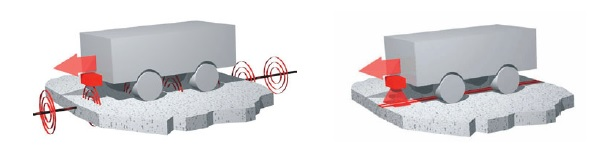
\includegraphics[width=0.9\textwidth]{Prinzipskizze_induktiven.jpg}
	\caption{Prinzipskizze zur induktiven und optischen Spurf\"uhrung (Quelle: G\"unter Ullrich, 2011 S. 79)}
	\label{Prinzipskizze_induktiven}
\end{figure}  
	\item \textbf{Orientierung durch Magnetmarken:} Eine weitere M\"oglichkeit der Steuerung ist die Abtastung von Magnetstreifen oder magnetischen Markierungen auf der Straßenoberfl\"ache. Dabei bedarf es zur Berechnung der Leitlinie einerseits der Koppelnavigation, zus\"atzlich der f\"ur die Peilung in regelm\"a\"ssigen Abst\"anden in den Boden eingelassenen Marken. Diese Marken k\"onnen rein passive Dauermagnete oder aber quasi-aktive Transponder sein (G\"unter Ullrich, 2011 S. 80). Das Bild \ref{Prinzipskizze_Koppelnavigation_rechts} ist eine Repr\"asentation der Navigation durch Magnetstreifen.
	\begin{figure}[h!]
		\centering
			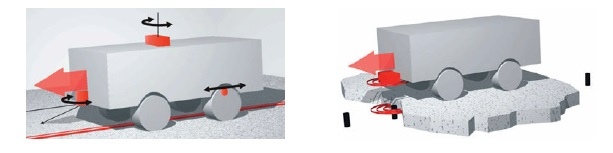
\includegraphics[width=0.9\textwidth]{Prinzipskizze_Koppelnavigation_rechts.jpg}
			\caption{Prinzipskizze zur Koppelnavigation (links) und zur Magnet- bzw. Transpondernavigation (rechts) (Quelle: G\"unter Ullrich, 2011 S. 79)}
			\label{Prinzipskizze_Koppelnavigation_rechts}
	\end{figure}	
	\item Bei der Lasernavigation bestimmt der Laserscanner die Position des FTF, dazu kommen noch optische Sensoren f\"ur Hinderniserkennung z.B. Mensch. Lasergef\"uhrte FTS bieten einen hohen Wert an Flexibilit\"at, da sie ohne Bodeninstallation funktionieren. Nur bei engerem Raum, kann die Lasernavigation nicht so effizient wie z.B. eine induktive Spurf\"uhrung sein, wenn viele Fahrzeuge zum Einsatz kommen. Um die Systemvorteile eine Lasernavigation optimal zu benutzen, ben\"otigt man allerdings ein passendes Anlagenkonzept. Die wichtigen Kriterien sind: die Einbindung in den gesamtbetrieblichen Materialflusssystem, die Anpassung an die vorhandenen Steuerungshierarchien und die optimale Auslegung der Technik in Bezug auf Fahrzeugbauart, Lastaufnahmemittel, Energiekonzept, Kommunikation und Leitsystem. Ein Aspekt, der f\"ur das Laser-gef\"uhrte FTS spricht, ist die Wirtschaftlichkeit. Und dies trotz der Alternativen Elektro-, Low-Cost- sowie induktiv gef\"uhrtes FTS. Letztere lassen sich so einrichten, dass sie auch auf leitdrahtlosen, rein rechnergef\"uhrten Teilstrecken verkehren k\"onnen. Keinerlei kostenintensive Bodeninstallation ben\"otigt dagegen das \"uber Lasersensor gesteuerte, v\"ollig frei navigierende Laser-FTS. Die Fahrzeuge orientieren sich lediglich an im Raum verteilten Reflektoren und mit Hilfe der Kombination von Winkel- und Distanzmessung. (Werner Swoboda, Industrie Anzeiger). Das Bild \ref{Prinzipskizze_Koppelnavigation_links} ist eine Visualisierung der Lasernavigation.
	\begin{figure}[h!]
		\centering
		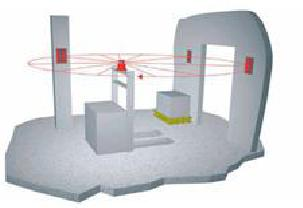
\includegraphics[width=0.8\textwidth]{Prinzipskizze_Koppelnavigation_links.jpg}
		\caption{Prinzipskizze zur Koppelnavigation (links) und zur Magnet- bzw. Transpondernavigation (rechts) (Quelle: G\"unter Ullrich, 2011 S. 79)}
		\label{Prinzipskizze_Koppelnavigation_links}
	\end{figure}

	\item \textbf{Orientierung durch GPS:} Seine Anwendung im Bereich der Fahrzeugsteuerung wird in Form des DGPS eingesetzt, die als Referenzsignal dient. DGPS bedeutet differential GPS und meint die Verwendung eines zus\"atzlichen GPS-Empf\"angers, der nicht auf dem FTF, sondern station\"ar fest installiert ist. Mit Hilfe dieses ortsfesten GPS-Empf\"angers wird der sich zeitlich \"andernde Fehler ermittelt, der dem GPS-System eigen ist. Mit Hilfe dieser Kenntnis k\"onnen zeitgleich die fahrenden GPS-Empf\"anger auf den FTF exakte Positionen ermitteln (Quelle: G\"unter Ullrich, 2011 S. 27). Diese Navigationstechnik braucht eine freie Sichtkegel von 15 Grad  nach oben (siehe Bild 4), m zuverl\"assig arbeiten zu k\"onnen. DieSchritte zur Erlangung der erforderlichen Fahr- und Positioniergenauigkeit sind:
	\begin{itemize}
		\item Pr\"ufung der \"ortlichen Gegebenheiten, insb. der Empfangsst\"arken der Satelliten
 \item Einsatz des Differential-GPS
 \item Real Time Kinematic Differential GPS. 
\end{itemize}
	\begin{figure}[h!]
		\centering
		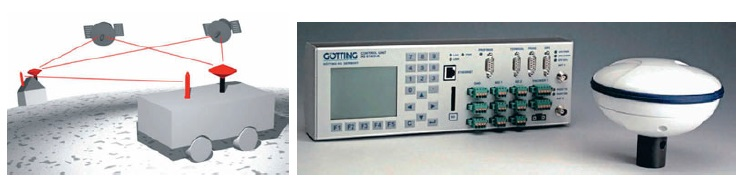
\includegraphics[width=0.9\textwidth]{Prinzipskizze_zur_Navigation_mittels_GPS.jpg}
		\caption{Prinzipskizze zur Koppelnavigation (links) und zur Magnet- bzw. Transpondernavigation (rechts) (Quelle: G\"unter Ullrich, 2011 S. 79)}
		\label{Systemarchitektur_FTS}
\end{figure}
Im Rahmen des Projekt FAISE wird die Navigation durch den Laser durchgef\"uhrt. Es kann hier kein Global Positioning System (GPS) verwendet werden, da das ganze Experiment in einem geschlossenen Raum gemacht wird. Weiterhin es kann auch keine Navigation durch die physische Leitlinie oder durch die St\"utzpunkte im Boden erzielt, weil der Boden gebrochen werden m\"usste.
\end{itemize}

\subsubsection{Steuerungstechnik}
Die interne Materialflusssteuerung ist eine Vorstufe der Transportauftragsabwicklung und wird nur dann ben\"otigt, wenn die Transportauftr\"age nicht klar dezidiert \"ubertragen, sondern aufbereitet werden m\"ussen. Eine Anforderung wie z. B. ben\"otige Ware A an Maschine B erfordert eine Umsetzung in einen oder mehrere Transportauftr\"age nach dem klassischen Muster. Hole von C und Bringe nach D. Die FTS-interne Materialflusssteuerung kombiniert also Quelle und Senke \"uber die in ihr hinterlegten Transportbeziehungen zu einem Transportauftrag und schickt diesen zur Durchf\"uhrung an die Transportauftragsverwaltung. Diese ganze Transportauftragsverwaltung ist in der FTS-Leisteuerung geregelt. 
Die FTS-Leitsteuerung ist die Kommandozentrale, um das FTS in das Umfeld zu integrieren. Au\"sserdem steuert es die FTF, die sich im System befinden. Damit ist das FTS dann in der 
Lage, die ihm \"ubertragenen Auftr\"age zu erf\"ullen. "`Eine FTS-Leitsteuerung besteht aus Hard- und Software. Kern ist ein Computerprogramm, das auf einem oder mehreren Rechnern abl\"auft. Sie dient der Koordination mehrerer Fahrerloser Transportfahrzeuge und/oder \"ubernimmt die Integration des FTS in die innerbetrieblichen Abl\"aufe."' (VDI 4451). Die Leitsteuerung bringt das FTS in seinem Umfeld zusammen, bietet seinen Bedienern vielf\"altige Service-M\"oglichkeiten und nimmt Transportauftr\"age entgegen. Weiterhin stellt sie den Aufgaben entsprechende Funktionsbl\"ocke zur Verf\"ugung. 
Die FTS-Leitsteuerung ist der Kern der FTS. In Rahmen des Projekt FAISE, wird es auch eine Leisteuerung ben\"otigt. Eine Leitsteuerung ist nur mit Hilfe eine Systemarchitektur zu implementieren und zu verstehen. In seinem Buch Fahrerlose Transportsysteme, hat G\"unter Ulrich zwei verschiedene Systemarchitekturen dargestellt. Eine f\"ur eine einfache FTS und eine andere f\"ur eine komplexe FTS. Da es bei FAISE nur mit vier FTF gearbeitet wird, ist es sinnvoll mit einer einfachen Systemarchitektur zu arbeiten. Das Bild 3 ist eine Repr\"asentation einer einfachen Systemarchitektur.
	\begin{figure}[h!]
		\centering
		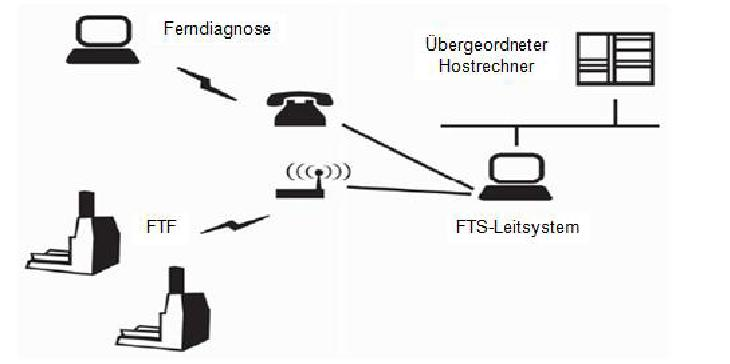
\includegraphics[width=0.9\textwidth]{Systemarchitektur_FTS.jpg}
		\caption{Die Systemarchitektur eines einfachen FTS (Quelle: G\"unter Ullrich, 2011 S. 93)}
		\label{Systemarchitektur_FTS}
	\end{figure}

Es gibt eine geringe Anzahl von FTF, mit denen die Leitsteuerung per WLAN in Verbindung ist. Au\"sserdem gibt es ein LAN, \"uber das es eine direkte Verbindung mit einem \"ubergeordneten Rechner gibt, von dem die Transportauftr\"age kommen. \"uber die angedeutete Telefonleitung ist eine VPN-Verbindung zur Ferndiagnose eingerichtet. Die Daten\"ubertragung zu den \"ubergeordneten Host-Rechnern erfolgt meist \"uber lokale, Ethernet basierte Netzwerke mit dem Protokoll TCP/IP. Solche Host-Rechner k\"onnen beispielweise Materialflusssteuerungssysteme zur Produktionssteuerung (z. B. SAP) Produktionsplanungssysteme (PPS) Lagerverwaltungssysteme (LVS) sein.“( vgl. G\"unter Ullrich, 2011 S. 96). 
Au\"sserdem nach der VDI 4451(Blatt 3) „zum internen Umfeld der FTF-Steuerung geh\"oren das Lastaufnahmemittel (LAM), Sensoren und Aktoren, Bedienfeld am Fahrzeug und das Sicherheitssystem. Das externe Umfeld besteht aus der FTS-Leisteuerung, anderen FTF, automatischen Stationen und Geb\"audeeinrichtungen“. Die Abbildung 1 stellt eine Darstellung eine FTF-Steuerung und ihr Steuerungsumfeld dar.
	\begin{figure}[h!]
		\centering
		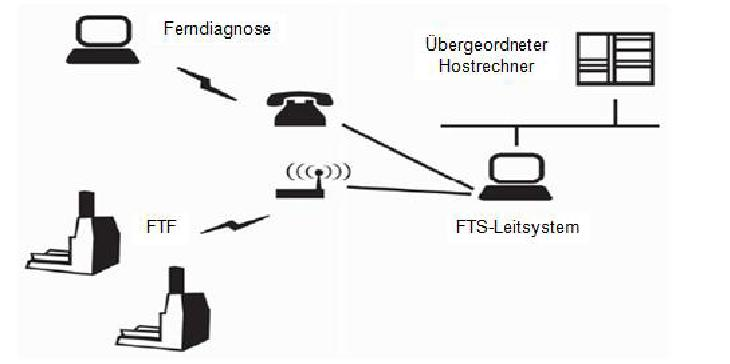
\includegraphics[width=0.9\textwidth]{Systemarchitektur_FTS.jpg}
		\caption{Allgemeine Darstellung einer FTF-Steuerung mit Datenschnittstellen (vgl. VDI 4451)}
		\label{Wertschoepfungskette}
	\end{figure}
Die administrative Ebene, die h\"aufig \"uber einen station\"aren Leitrechner realisiert wird, verwaltet die Transportauftr\"age der ganzen Materialflusssteuerung. Die operative Ebene, die auch als Fahrzeugsteuerung bezeichnet wird, erh\"alt ihre Informationen \"uber die Fahrzeugdisposition der administrativen Ebene. Der Funktionsblock Kommunikation leitet den stattgefundenen Datenaustausch zum Manager weiter. Dieser sorgt f\"ur die Koordination, indem er die Fahrauftr\"age in einzelne Befehle aufteilt, sowie f\"ur ein reibungsloses Zusammenwirken der einzelnen Funktionsbl\"ocke. Neben dem Block Kommunikation sind weitere Bl\"ocke vorhanden. Dazu geh\"ort f\"ur die gesamte Last\"ubergabe inklusive der Lastlagererfassung verantwortliche Lastaufnahme, das Energiemanagement, welches den Lade- und Allgemeinzustand der Batterien \"uberwacht, und der Block \"uberwachung/Sicherheitsschnittstelle, welcher zum Schutz der Personen und Sachgegenst\"ande dient. Der Funktionsblock Fahren und die damit verbundene Sensorik bzw. Aktorik koordinieren die Ablaufsteuerung der Funktionen des Orientierungssystems (Langenbach Maik, 2012, S. 33).

\subsection{Materialflusssysteme}
Damit ein Produkt auf den Markt kommen kann, muss man ihn denken, ihn erstellen und dann ihn vermarken. Die Produkterstellung und -vermarktung sind Prozesse des Wirtschaftens. Vorprodukte oder Materialen werden von Beschaffungsm\"arkten in die Unternehmen gef\"uhrt und dort werden sie durch besondere Produktionsprozesse transformiert. Am Ende der Produktion, steht ein Endprodukt, der f\"ur den Konsum bereits ist. 
Die Produktion und Logistik von G\"utern sind daher sehr wichtige Bereiche f\"ur den Unternehmenserfolg. Allerdings f\"uhren heute die unterschiedlichen Auspr\"agungen der Logistik z.B. in Produktions-, Handels-, oder Verkehrsunternehmen zu einer terminologischen Differenzierung der Logistik. Der Materialflussbegriff leitet sich einfach von dem logistische Konzept ab, in anderen W\"ortern das Materialflusssystem f\"uhrt in der Logistik zur\"uck. Die Abbildung 2. dient zur Erl\"auterung einer konventionellen Wertsch\"opfungskette. 
	\begin{figure}[h!]
		\centering
		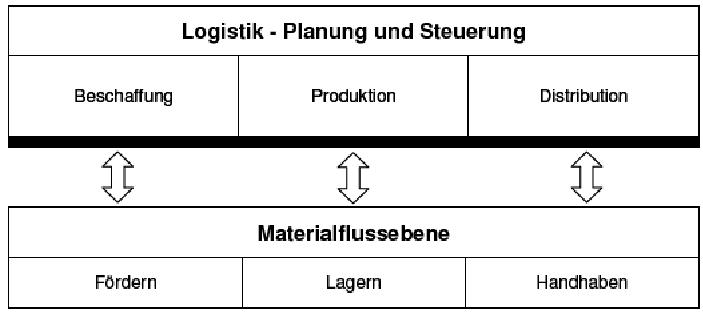
\includegraphics[width=0.9\textwidth]{Wertschoepfungskette.jpg}
	\caption{Elemente einer Wertsch\"opfungskette (vgl. Wulz, J, 2008, S. 7)}
	\label{Wertschoepfungskette}
\end{figure}

Der Begriff Materialfluss bedeutet die Verkettung aller Prozesse bei der Beschaffung, Bearbeitung, Verarbeitung sowie bei der Distribution von G\"utern innerhalb festgelegter Bereiche. Deswegen l\"asst sich der Materialfluss in vier Stufen unterordnet: externer Transport, betriebsinterner Materialfluss, geb\"audeinterner Materialfluss und Materialfluss am Arbeitsplatz. Nach dem Verein Deutscher Ingenieur bzw. VDI-241 beinhaltet die Logistik f\"unf Hauptfunktionen. Diese Funktionen sind Bearbeiten, Pr\"ufen, Handhaben, F\"ordern, Lagern und Aufenthalten. Neben diesen Hauptfunktionen z\"ahlen auch Nebenfunktionen wie z.B. Montieren, Umschlagen, Kommissionieren, Palettieren und Verpacken (VDI 2411). Jedoch ist auf der Ebene des Materialflusssystems nur drei Funktionen zu ber\"ucksichtigen: F\"ordern, Lagern, Handhaben. Die anderen Funktionen setzen sich normalerweise aus den erl\"auterten Funktionen zusammen. Dieses Arbeitsteil wird in zwei Teile gegliedert. Im ersten Teil werden die drei Funktionen der Materialflusssysteme vorgestellt Im zweiten Teil wird eine Planung von Materialflusssystemen dargestellt.

\paragraph{Funktionen von Materialflusssystemen}
\begin{itemize}
	\item \textbf{Funktion F\"ordern} \\
	F\"ordern bedeutet Transportieren und ist eine der wichtigsten Aspekte innerhalb des Materialflusssystems. Nach der VDI 2411 ist F\"ordern das Fortbewegen von Arbeitsgegenst\"anden in einem System. „Die Fortbewegung oder Ortver\"anderung von G\"utern oder Personen mit technischen Mitteln wird allgemein als Transport bezeichnet. Findet diese Ortsver\"anderung in einem r\"aumlich begrenzten Gebiet wie beispielsweise innerhalb eines Betriebes oder Werkes statt, so wird dieser Vorgang durch den Begriff F\"ordern pr\"azisiert. Das F\"ordern bzw. die F\"ordertechnik umfasst also das Bewegen von G\"utern und Personen \"uber relativ kurze Entfernungen einschlie\"sslich der dazu notwendigen technischen organisatorischen und personellen Mittel“(Ten Hompel, Schmidt, Nagel, 2007, S. 119). 
Das F\"ordermittel (technisches Transportmittel, zur Ortsver\"anderung von G\"utern oder Personen) und das F\"orderelement bilden das physikalische Bestandteil eines F\"ordervorgang. Der Ablauf und die Steuerung werden durch den F\"ordervorgang dargestellt. In Punkto F\"ordermittel kann auf verschiedenste Elemente der Materialflusstechnik zur\"uckgegriffen werden. Dies umfasst unter anderen Rollenbahnen, und FTS. Neben der M\"oglichkeit auf automatisierte F\"ordermittel zur\"uckzugreifen, kommen auch manuell mechanisierte bzw. rein manuelle Systeme zum Einsatz. In diesem Fall ist der Mensch oder der Bediener eines F\"ordermittels wesentlich f\"ur den Ablauf eines reibungslosen Materialflusses in Zusammenspiel mit den physikalischen Elementen sowie dem Prozessablauf verantwortlich. (Wulz, J, 2008, S. 8). Das Bild 4 gilt als Beispiel eines F\"ordersystems. 
	\begin{figure}[h!]
	\centering
  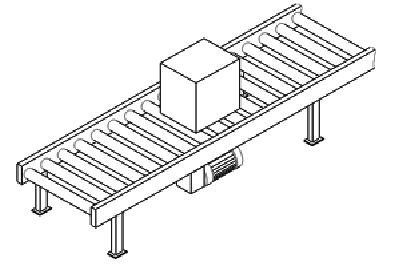
\includegraphics[width=0.7\textwidth]{Stetigfoerderer.jpg}
	\caption{Beispiel eines Stetigf\"orderer (entnommen aus Ten Hompel, Schmidt, Nagel, 2007, S. 131)}
	\label{Stetigfoerderer}
\end{figure}

\item \textbf{Funktion Lagern} \\
Das Lagern ist jedes geplante Liegen des Arbeitsgegenstandes im Materialfluss. Das Lager ist ein r\"aumlich abgegrenzter Bereich bzw. eine Fl\"ache zum Aufbewahren von St\"uck- und/oder Sch\"uttg\"utern in Form von Rohmaterialien, Zwischenprodukte oder Endprodukte, das mengenm\"a\"ssig erfasst wird (VDI-2411). Die Einlagerung von Lagereinheiten, die Aufbewahrung und Bereithaltung von Lagereinheiten auf Lagerpl\"atzen und die Auslagerung einer Lagereinheit, sind die grundlegenden Prozesse in einem Lager.
Aufgrund der starken Ver\"anderungen im Markt, m\"ussen auch die unternehmerischen Abl\"aufe an Lagersysteme schnell angepasst werden. In einem Lagersystem werden im Verlauf des Materialflusses Speicher- bzw. Lagerfunktionen sowie F\"orderfunktionen wahrgenommen. 
Aufgabe eines Lagers ist das Bevorraten, Puffern und Verteilen von G\"utern. W\"ahrend Vorratslager lang- und mittelfristige und Pufferlager kurzfristige Bedarfsschwankungen ausgleichen sollen, erf\"ullen Verteillager neben der Bevorratungs- noch eine Kommissionierfunktion. Daher k\"onnen die Aufgaben eines Lagers anhand folgender Ausgleichsma\"ssnahmen beschrieben werden: Zeitausgleich, Mengenausgleich, Raumausgleich und Sortimentsausgleich. (Stich, V.; Bruckner, A.; 2002). Ein Zeitausgleich ist immer dann erforderlich, wenn die Zeitfunktion der Nachfrage nicht der Zeitfunktion der Produktion entspricht. Beispielsweise steht eine losgr\"o\"ssenoptimierte Fertigung einer saisonalen Nachfrage gegen\"uber. Gerade in Bereichen mit Serienfertigung, in denen aus Kostengr\"unden in der Regel gr\"o\"ssere Mengen als die Nachfragemengen produziert werden, muss Mengenausgleich vollzogen werden. Sobald der Produktionsort nicht mit dem des Produktabnehmers \"ubereinstimmt, findet mit Hilfe von Verkehrstr\"agern ein Raumausgleich statt. Mit zunehmender Sortimentsbreite steigt die Wahrscheinlichkeit, dass die Anzahl der Produktionsstandardorte steigt. (Lagenbach, M, 2012, S. 14).

\item \textbf{Funktion Handhaben } \\
Der Begriff Handhaben wurde gedanklich von de menschlichen Hand abgeleitet, wird aber auch f\"ur automatische ablaufende Vorg\"ange zur Manipulation von Objekten gebraucht. Handhaben bedeutet etwas greifen, bewegen und an einem bestimmten Ort ablegen. Das hei\"sst, durch Handhaben wird die Lage oder Position von Objekten ge\"andert. Im \"ubertragenen Sinne bedeutet handhaben auch bewerkstelligen bzw. praktisch aus\"uben. Von Handhabungstechnik spricht man, wenn f\"ur die Handhabung Ger\"ate eingesetzt werden. 
Die Richtline VDI 2860 definiert die Funktion Handhaben als „das Schaffen, definiertes Ver\"andern oder vor\"ubergehendes Aufrechterhalten einer vorgegebenen r\"aumlichen Anordnung von geometrisch bestimmten K\"orpern.“ Die Teilfunktionen des Handhabens stellen das Speichern, das Bewegen, das Sichern, das Kontrollieren und das Ver\"andern von G\"utern dar. Das Handhaben kann sowohl als eine Funktion als auch eine Fertigung des Materialflusses betrachtet werden. Eine m\"ogliche Handhabungsfunktion im Materialfluss ist z.B. das Palettieren, worunter die Stapelung von St\"uckg\"utern zu einem St\"uckgutstapel nach einem gewissen Muster verstanden wird. Handhabungsfunktionen k\"onnen entweder von Automaten z.B. Roboter oder von Menschen durchgef\"uhrt werden. Auf Grund der Greifflexibilit\"at ist der Mensch jedoch meist un\"ubertroffen in der Handhabung.
\end{itemize}

\subsection{Fallbeispiele}
\subsubsection{FTS in der Gl\"asernen Manufaktur Dresden (Volkswagen)}
Volkswagen AG montiert das neue Modell der Luxusklasse "Phaeton" in der "Gl\"asernen Manufaktur" in Dresden. Die Materialversorgung \"ubernimmt ein fahrerloses Transportsystem mit 56 frei navigierenden Fahrzeugen. Die gesamte Steuerungs- und Navigationstechnik stammt von FROG Navigation Systems, dem Projektpartner des Generalunternehmers AFT (Mechanik).
Die Produktion ist auf drei Ebenen unterteilt: . Die eigentliche Montage findet auf den beiden oberen Montageebenen statt: Die Rohrkarosse befindet sich auf einer Montageplattform, die Teil des Schuppenbandes ist, das sich sicher in den Hallenboden einf\"ugt und mit konstanter Geschwindigkeit durch die Montagezyklen bewegt. Danach erfolgt die \"ubergabe an eine schwere Elektroh\"angebahn (EHB) zur H\"angemontage. W\"ahrend der H\"angemontage erfolgt die Hochzeit, d. h. das Zusammenf\"ugen von Karosse und Triebsatz, wobei der Triebsatz von einem Fahrerlosen Transportfahrzeug (FTF) herangebracht wird. Anschlie\"ssend wird die Karosse wieder auf eine Schubplattform, die sog Schuppe, zur Komplettierung und Qualit\"atskontrolle gestellt.

Im Untergeschoss, der Logistikebene, wird die verbauende Ausr\"ustung zur Verf\"ugung gestellt und in Betrieb genommen. Die FTS \"uberminnt die Versorgungsleitungen der Materialien und damit eine erhebliche logistische Funktion . Um zwischen den Ebenen zu wechseln, nutzen die  automatischen Fahrzeug-Hebeb\"uhnen .
Das FTS hat die grunds\"atzliche Aufgabe, die Montagelinien (Schuppenband oder EHB) zu versorgen. Dabei wird allerdings zwischen folgenden sechs Gewerken unterschieden:
\begin{itemize}
\item[1.] Anlieferung von Warenk\"orben auf die Schuppe
\item[2.] Anlieferung von Schalttafeln (Cockpits)
\item[3.] Anlieferung von Kabelstr\"angen
\item[4.] Anlieferung des Triebwerks mit Fahrwerk und Ausf\"uhrung der Hochzeit
\item[5.] Anlieferung von Warenk\"orben zur H\"angemontage
\item[6.] Anlieferung der T\"uren plus Warenk\"orbe
\end{itemize}
\subsubsection{FTS beim Automobilhersteller BMW im Werk Leipzig}
Das BMW-Werk in Leipzig hat im Jahre 2005 mit der Produktion der 3er reihe (E90) gestartet
Im Bereich der Teileversorgung \"ubernimmt erstmals in der Geschichte der Automobilindustrie ein Fahrerloses Transportsystem (FTS) umfangreiche Logistikfunktionen. Folgende Prozesse wurde f\"ur die Teilversorgung im Leipzig-Werk definiert:

\begin{itemize}
\item Direktanlieferung per LKW: Gro\"sse Teile mit geringer Komplexit\"at (z. B. Bodenmatte oder Kofferraumverkleidung) werden per LKW zeitnah und in unmittelbare N\"ahe des Verbauortes angeliefert.
\item Modulanlieferung per EHB8: Gro\"sse und komplexe Baugruppen (z. B. Cockpit) werden direkt auf dem Werksgel\"ande von externen Lieferanten oder BMW Mitarbeitern montiert.
\item Lagerware per FTS: Die Mehrzahl der Teile wird in einem Versorgungszentrum gelagert, kommissioniert und mit Fahrerlosen Transportfahrzeugen (FTF) an die jeweiligen Verbauorte in der Montage gebracht (G\"unter Ullrich, 2011 S. 36).\end{itemize}
Es sind 74 FTF im Einsatz, als Ladehilfsmittel werden mehr als 2.000 Rollwagen in zwei unterschiedlichen Ausf\"uhrungen eingesetzt. Je FTF werden entweder zwei kleine Rollwagen, zur Aufnahme von Beh\"altern bis DIN-Gr\"o\"sse, oder ein so genannter \"ubergro\"sser Rollwagen zur Aufnahme von Gro\"ssbeh\"altern eingesetzt. Zus\"atzlich gibt es noch die Sequenziergestelle mit Sonderaufbauten (G\"unter Ullrich, 2011 S. 37). Durch einen Laser-Scanner auf dem FTF wird den Personenschutz und Hinderniserkennung \"ubernommen. 

Die Fahrerlosen Transportfahrzeuge finden ihren Weg mit Hilfe der so genannten freien Navigation. Damit ist gemeint, das die Fahrzeuge ohne physikalische Leitspuren und nach einem kombinierten Prinzip aus Kopplung und Peilung arbeiten. Kopplung bedeutet die Auswertung von fahrzeuginternen Sensoren (Messr\"ader und ein faseroptischer Kreisel), wodurch der zur\"uckgelegte Weg samt Kurven bestimmt wird (G\"unter Ullrich, 2011 S. 37). Bei jeder Peilung werden aufgetretene Fahrfehler, die durch Schlupf der R\"ader oder durch Ver\"anderungen des Raddurchmessers auftreten k\"onnen, korrigiert. Die Vorteile dieses, auch Magnet Navigation genannten, Verfahrens liegen in der Zuverl\"assigkeit und der Flexibilit\"at bei zuk\"unftigen Layoutanpassungen (G\"unter Ullrich, 2011 S. 37).



	
	% Chapter 3 Projektorganisation
	\clearpage
	\ohead[Projektorganisation]{Projektorganisation}
	\chead[Uni Oldenburg]{Uni Oldenburg}
	\ihead[PG FAISE]{PG FAISE}
	\setheadtopline{1pt}
	\setheadsepline{0.5pt}
	\ofoot[Endbericht]{Endbericht}
	\cfoot[\pagemark]{\pagemark}
	\ifoot[30. September 2014]{30. September 2014}
	\setfootsepline{0.5pt}
	\setfootbotline{1pt}
	\section{Projektorganisation}
Die nachfolgenden Abschnitte beschreiben den organisatorischen Ablauf innerhalb der Projektgruppe. Dazu geh\"ort die Aufteilung in Gruppen, sowie die zeitliche Planung und Rollenverteilung. Des weiteren werden hier das Vorgehen f\"ur das gesamte Projekt und die verwendeten Werkzeuge beschrieben.

\subsection{Organisation der Teilgruppen (Materialfluss, Fahrzeuge, Simulation)}
Die Projektgruppe ist in die drei Teilgruppen unterteilt,  da das Gesamtprojekt in eindeutig abgrenzbare Aufgabenfelder gegliedert ist und so Kompetenzen und Verantwortlichkeiten klar definiert werden können. 

\begin{itemize}
\item \textbf{Materialfluss} \\
Die Teilgruppe Materialfluss befasst sich mit Programmierung der Sensorik und Aktorik für die Rampen, sowie dem Aufbau eines Sensornetzwerkes zur Kommunikation zwischen den verschiedenen Akteuren der Simulation. 

\item \textbf{Fahrzeuge} \\
Die Teilgruppe Fahrzeuge befasst sich mit allen Aspekten, die für das Funktionieren der Fahrzeuge verantwortlich sind. Dazu zählen unter anderem die Navigation, Odometrie und Lokalisierung. Auch ist die Einrichtung der Versorgungsinfrastruktur für die Fahrzeuge in Form von Ladestationen f\"allt in den Aufgabenbereich der Fahrzeuggruppe. Zusammen entwickeln die Teilgruppen Fahrzeuge und Materialfluss das physische System, so dass Kommunikation und Abstimmung zwischen diesen beiden Gruppen besonders wichtig sind. 

\item \textbf{Simualtion} \\
Die Teilgruppe Simulation entwickelt die Software mit der eine virtuelle Simulation erstellt wird. Diese Software beinhaltet einen hybriden Modus, in dem das physische System auf die Software abgebildet wird und beide Teilsysteme ein Gesamtsystem bilden. Für die Entwicklung des Hybridmodus muss ein funktionierendes physisches System vorliegen.
\end{itemize}

\subsection{Rollenverteilung}

Um organisatorische Aspekte innerhalb des Projektes besser umsetzen zu k\"onnen, wurden unterschiedliche Rollen definiert, die jeweils einen Bereich des Projektes abdecken sollen. Dazu geh\"oren folgende Aufgaben:

\begin{itemize}
\item\textbf{Administrator}

Der Administrator ist f\"ur die Einrichtung und Betreuung der Server und Tools zust\"andig, dazu z\"ahlt auch die Einrichtung der Webseite.

\item \textbf{Aussendarstellung}

Um das Projekt vern\"unftig zu Repr\"asentieren, verwalten die zust\"andigen der Aussendarstellung den Inhalt der Webseite. Ausserdem sind sie f\"ur die externen Kontakte und Events / Pr\"asentationen verantwortlich.

\item \textbf{Dokumentenbeauftragte}

Damit am Ende ein einheitliches Format f\"ur den Endbericht gilt, organisieren, sammeln und verwalten die Beauftragten jegliche Quellen und Berichte ( dazu z\"ahlt auch das Repository ). Des weiteren sind sie Ansprechpartner bei fragen zur Literatur.

\item \textbf{Gruppenleiter}

Da das Projekt aus drei Teilgruppen besteht, besitzt jede Gruppe einen eigenen Gruppenleiter, der die Prozesse innerhalb der Gruppe lenkt und gemeinsam mit den anderen Gruppenleitern das gesamte Projekt koordiniert.

\item \textbf{Qualit\"atsmanagement}

Damit der Projektplan eingehalten wird, ist es Aufgabe des Qualit\"atsmanagements, dass die Prozesse ( Scrums ) eingehalten und korrekt ausgef\"urt werden. Zus\"atzlich sind sie f\"ur die System und Integrationstests verantwortlich.

\item \textbf{Werkzeugbeauftragte}

Die Werkzeugbeauftragen verwalten die ben\"otigten Ger\"ate und Schl\"ussel f\"ur die gesamte Projektgruppe. Weiterhin regeln sie, mit R\"ucksprache mit den Betreuern, den Einkauf der Hardware und Software.

\end{itemize}


\subsection{Vorgehensmodell}
Für die Durchführung der Projektgruppe muss ein Vorgehensmodell, sowohl für die Gesamt- als auch für die Teilgruppen, festgelegt werden. Durch ein Vorgehensmodell wird die Arbeit im Team strukturiert und es wird festgelegt, wie bestimmte Aufgaben, wie z.B. Abgleich mit Kunden und Anwendern, umgesetzt werden sollen. Sowohl für die Teilgruppen als auch für die Gesamtgruppe wurde ein Scrummodell als Vorgehensmodell gewählt ( siehe Abbildung 9).

	\begin{figure}[h!]
		\centering
			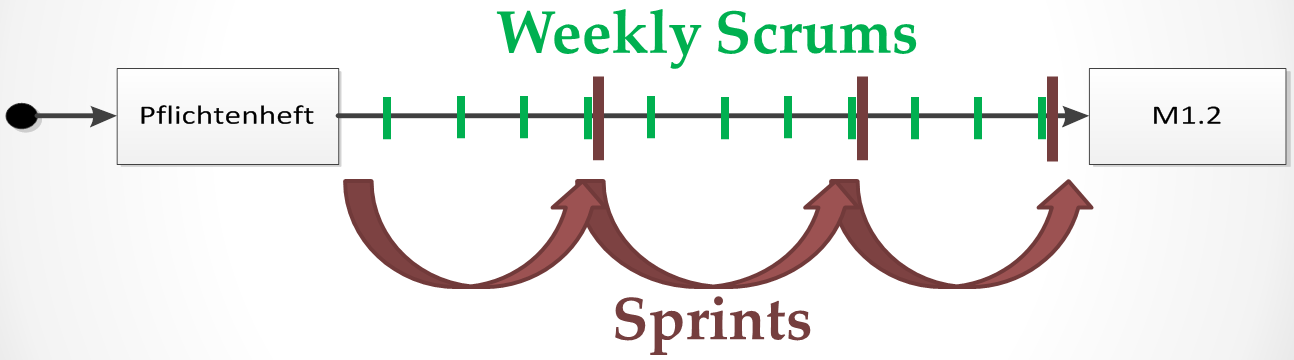
\includegraphics[width=0.9\textwidth]{Projektorganisation_Scrum.png}
			\caption{Scrumplanung f\"ur einen Meilenstein}
			\label{Projektorganisation_Scrum}
	\end{figure}	

Da es für ein sehr komplexes Projekt, wie das vorliegende, schwierig ist nur von einer groben Vision, sowie von User Stories auszugehen, wurden zun\"achst auf Basis des vorliegenden Lastenhefts in jeder Teilgruppe Pflichtenhefte erstellt. Anschließend wurden die dazugeh\"origen User Stories definiert, die die Anforderungen aus dem Pflichtenheft ber\"ucksichtigen und aus Anwendersicht darstellen. Die Sprints in den Teilgruppen sind mit einem Monat bemessen und werden zur Durchf\"uhrung der User Stories genutzt. Die Rolle des Product Owners wird von den beiden Betreuern eingenommen, die sowohl für die Teil- als auch für die Gesamtgruppen zur Verfügung stehen, um die entwickelten Funktionalit\"aten abzugleichen.
Die Durchf\"uhrung von Daily Scrums ist zeitlich nicht m\"oglich, da es sich um eine studentische Projektgruppe handelt, deren Stundenplan keine t\"aglichen Treffen erm\"oglicht. Deshalb wurde das Scrum Vorgehensmodell dahingehend angepasst, dass die Daily Scrums in Weekly Scrums abgewandelt wurden. Die Weekly Scrums finden sowohl in den Teilgruppen als auch in der Gesamtgruppe statt. In den Weekly Scrums der Gesamtgruppe wird zun\"achst von jeder Person berichtet, welche Aufgaben in der vorherigen Woche erledigt wurden, damit entstandene Probleme und Hindernisse direkt in der Gruppe besprochen und eventuell beseitigt werden k\"onnen. Die Ergebnisse aus den Teilgruppen werden ebenfalls vorgestellt und mit den Product Ownern abgeglichen.
Das Scrum Vorgehensmodell wird mit  Prototyping kombiniert ( siehe Abbildung 10 ).

Durch das Prototyping sollen zu bestimmten Meilensteinen die kombinierten Ergebnisse aus den Teilgruppen vorgestellt werden, um den Stand des Gesamtsystems begutachten zu k\"onnen. Betrachtet man das gesamte Projekt, so besteht es aus 2 Prototyping Phasen. Diese trennen sich im zweiten Meilenstein. Bis zu diesem Zeitpunkt wird mit horizontalen Prototyping die Basis des Projektes geschaffen. Das bedeutet, dass alle Grundfunktionalit\"aten implementiert und umgesetzt werden. Danach folgt das vertikale Prototyping in dem die Funktionalit\"aten um weitere Aspekte und Feinheiten er\"anzt werden. Innerhalb dieser beiden Phasen kommt es immer wieder zu Aufgabenbereichen, die jede Teilgruppe f\"ur sich umsetzt. Ebenfalls sind Phasen vorhanden, in denen die Ergebnisse der einzelnen Gruppen zusammengef\"uhrt werden m\"ussen, wodurch das Zusammenspiel zwischen dem Materialfluss und der Volksbots, sowie die Darstellung in der Simulation, entsteht.

	\begin{figure}[h!]
		\centering
			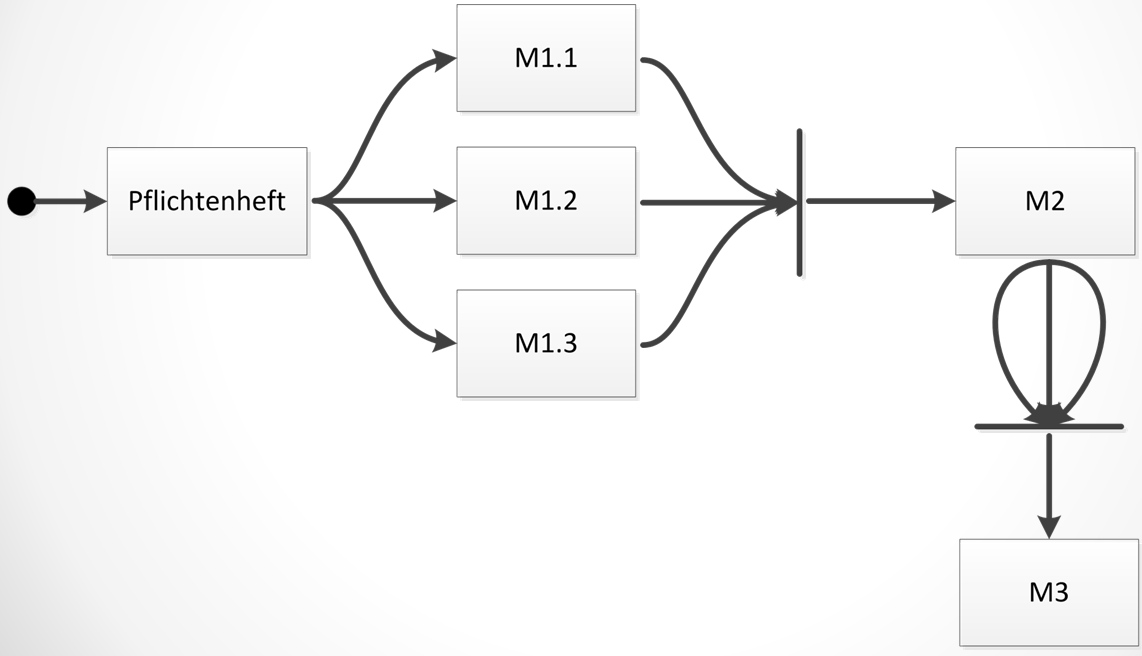
\includegraphics[width=0.9\textwidth]{Vorgehensmodell_Prototyping.png}
			\caption{Modell für die Darstellung der einzelnen Projektphasen}
			\label{Vorgehensmodell_Prototyping}
	\end{figure}	

\subsection{Werkzeuge}	

Zur Unterstützung der Zusammenarbeit in der Projektgruppe wurden verschiedene Werkzeuge ausgewählt um die Kollaboration zu vereinfachen. Um eine gute Verknüpfung der Werkzeuge zu gewährleisten, wurde versucht die Produkte aus einer Hand zu beziehen. Nach einiger Recherche, stachen zwei Möglichkeiten heraus. Entweder die Open-Source Software Redmine oder eine kommerzielle Lösungen von der Firma Atlassian.

Die beiden Lösungen wurden daraufhin auf Basis verschiedener Kriterien verglichen. Zu diesen Kriterien zählten mitunter Usability, Verbreitung am Markt, Stabilität und Wartbarkeit.

Die Evaluation ergab Atlassian als klaren Sieger und die Projektgruppe einigte sich im speziellen auf die Werkzeuge \textbf{Jira} und \textbf{Confluence}. 

\begin{figure}[h!]
		\centering
			
\includegraphics[width=0.5\textwidth]{logoAtlassian.png}
			\caption{Hersteller der Projektwerkzeuge}
			\label{Vorgehensmodell_Prototyping}
	\end{figure}

\subsubsection{Jira}
Jira ist ein Projektmanagement-Tool. Neben dem Verwalten von Vorgängen und Fehlern, lässt sich Jira mit einer \textit{Agile} Erweiterung sehr gut zum planen, steuern und verwalten von Sprints. Eine einfache Übersicht über die verschiedenen, anstehenden Aufgaben können die Projektmitglieder über die sogenannten Boards erhalten. Hier wird genau für die verschiedenen User Stories deren Fortschritt angezeigt und welches Projektmitglied gerade welche Aufgabe bearbeitet.

\subsubsection{Confluence}
Confluence ist ein Wiki welches sich sehr gut in Jira integriert. So muss die Benutzerverwaltung nur einfach in Jira eingerichtet werden. Confluence greift dann auf das Benutzerverzeichnis von Jira zurück. 

	
		% Chapter 4 Komponentenbeschreibung
	\clearpage
	\ohead[Komponentenbeschreibung]{Komponentenbeschreibung}
	\chead[Uni Oldenburg]{Uni Oldenburg}
	\ihead[PG FAISE]{PG FAISE}
	\setheadtopline{1pt}
	\setheadsepline{0.5pt}
	\ofoot[Endbericht]{Endbericht}
	\cfoot[\pagemark]{\pagemark}
	\ifoot[30. September 2014]{30. September 2014}
	\setfootsepline{0.5pt}
	\setfootbotline{1pt}
	\section{Komponentenbeschreibung}
\subsection{Mikrocontroller}
Ein Mikrocontroller ist ein kleiner Computer auf einem einzelnen Halbleiter-Chip. Dazu geh\"ort ein Prozessor, der Programme ausf\"uhren kann, Arbeits- und Programmspeicher sowie Schnittstellen, die eine Kommunikation mit der Umgebung erm\"oglichen sog. Peripheriefunktionen \cite{Wikibooks:2014:Online}. Mit ihnen lassen sich komplexe Aufgaben l\"osen, f\"ur die sonst ein aufw\"andiger Schaltungsaufbau notwendig w\"are. Standardm\"a{\ss}ig sind folgende Bestandteile in Mikrocontrollern integriert:
CPU, SRAM und Flash-Speicher f\"ur den Programmcode. Weiterhin bieten MCs analoge und digitale Ports, mehrere AD/DA-Wandler, Timer und Schnittstellen zur Kommunikation mit der Au\"{ss}enwelt \cite{Viktor:Seib:2014:Online}. In der nachstehenden Abbildung ist der allgemeine schematische Aufbau eines Mikrocontrollers in folgender Abbildung dargestellt.
\begin{figure}[h!]
	\centering
		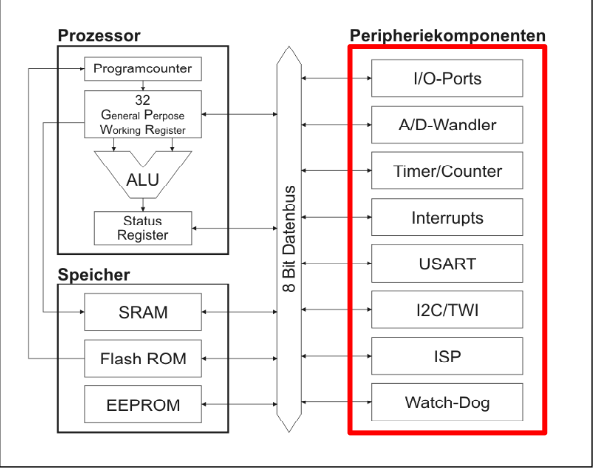
\includegraphics[width=0.9\textwidth]{Aubau_eines_Mikrocontrollers.png}
	\caption{schematischer Aufbau eines Mikrocontrollers \cite{habil:Ostermeye:2014:Online}}}
	\label{Aufbau eines Mikrocontrollers}
\end{figure}

\begin{itemize}
\item Prozessor (CPU)
\begin{itemize}
          \item Arithmetic Logic Unit kurz ALU (Rechenwerk)
          \item 32 GPIO-Register (Arbeitsregister f\"ur ALU)
          \item Programmcounter (Programmposition)
					\item Statusregister (Status der aktuellen Operation) 
\end{itemize}
\item Speicher
\begin{itemize}
          \item SRAM– Datenspeicher (Static Random-Access Memory)
					\item Flash ROM– Programmspeicher (Read Only Memory)
					\item EEPR OM– Festspeicher (Electrically Erasable Programmable Read-Only Memory)
\end{itemize}
\item Peripheriekomponenten
    \begin{itemize}
          \item I/O-Ports Prim\"arfunktion der Pins (Ein- und Ausg\"ange)
          \item A/D-Wandler (Einlesen von analogen Spannungen)
          \item Timer/Counter (Zeitintervall-/PBM-Generator)
					\item Interrupts (Programmunterbrechungsroutinen)
					\item USART, I2C/TWI und SPI (Kommunikationsschnittstellen)
					\item Watch-Dog (Absicherung gegen Systemfehler)
					\item ISP (Schnittstelle zum \"{u}bertragen des kompilierten Programms)
	\end{itemize}
\end{itemize}
Mikrocontroller sind im heutigen Leben weit verbreitet und es gibt eine viele Anzahl von Herstellern, die mikrocontroller anbieten. Im folgenden werden einige Hersteller mit ihren MC-Familien beispielhaft aufgef\"urt:
\begin{itemize}
\item Intel (8051-Serie)
\item Renesas (H8)
\item Zilog (Z8)
\item Microchip (Pic)
\item Freescale (fr¨uher Motorola) (68HC08 bzw. 68HCS08)
\item Atmel (AVR, 8051-Serie)
\end{itemize}
F\"ur das Projekt FAISE wurde das Atmel-Serie eingesetzt. Es sind Mikrocontroller mit erweiterten Peripherien und Funktionen, die auf der 8-Bit-AVR-Architektur basieren. Bei AVR handelt es sich um einen RISC-Kern, der an der Universit\"at von Trondheim in Norwegen entwickelt und von Atmel aufgekauft wurde. Die CPU besitzt 32 allgemeine 8-Bit Register (general purpose registers) und ist in der Lage in einem einzigen Taktzyklus Daten aus zwei beliebigen Registern in die ALU zu laden, diese zu verarbeiten und das Ergebnis in einem beliebigen Register zu speichern \cite{Viktor:Seib:2014:Online}. Die Konfiguration eines Atmega 8 der Firma Atmel sieht so aus:
\begin{figure}[h!]
	\centering
		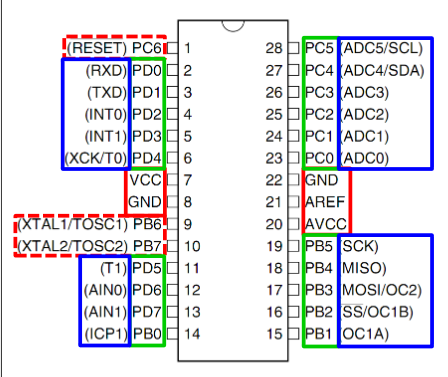
\includegraphics[width=0.9\textwidth]{Atmel8.png}
	\caption{Atmel 8 \\ \url{(http://www.ids.tu-bs.de/tl\_files/Lehre/Vorlesungen/Simulation2/Einfuehrung\_in\_die\_MC\_Programmierung\_Teil1.pdf)}}
	\label{Atmel 8}
\end{figure}
\begin{figure}[h!]
	\centering
		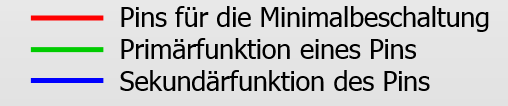
\includegraphics[width=0.9\textwidth]{LegendeAtmel8.png}
	\caption{Atmel 8 \URL{(http://www.ids.tu-bs.de/tl\_files/Lehre/Vorlesungen/Simulation2/Einfuehrung\_in\_die\_MC\_Programmierung\_Teil1.pdf)}}
	\label{Legende Atmel8}
\end{figure}
\begin{itemize}
\item Pins f\"ur die Minimalbeschaltung
\begin{itemize}
          \item Spannungsversorgung
          \item ReferenzspannungTaktgeber
          \item Reset      
					\end{itemize}
\item Prim\"arfunktion eines Pins
\begin{itemize}
          \item Ein- bzw. Ausgang
					\end{itemize}
\item Sekund\"arfunktion des Pins
\begin{itemize}
          \item A/D-Wandlereingang
          \item Ext. Interrupt
          \item PBM-Ausgang   
\end{itemize}
\end{itemize}
F\"ur die Programmierung der AVR-Controller gibt es eine kostenlose Entwicklungsumgebung AVR-Studio, die das Einbinden des Compilers problemlos erlaubt.

\subsection{Sensorik/ Aktorik}
Hauptziel der Teilgruppe Materialfluss ist das Management von Paketen auf einer Rampe. Die Aufgabe der Sensorik ist dabei, die mit Lichtschranken ausgestatteten Rampen Paketen zu detektieren und auf \"Anderung der Position der Paketen zu reagieren. Die Lichtschranken bestehen aus einer Lichtstrahlenquelle (dem Sender) und einem Sensor (dem Empf\"anger) f\"{u}r diese Strahlung. Als Lichtquelle kommt Infrarotlicht zum Einsatz und der Vorteil besteht in der einfachen Einstellung des Sensorsystems durch den sichtbaren Lichtfleck. Das Funktionsprinzip der Lichtschranke besteht darin, der zu  \"andernden Zustand durch die Lichtintensit\"at mit dem Sensor zu registrieren. 
Die Rampen werden auf Hardwareebene um eine Aktorik zum Arretieren der Kisten erg\"anzt. Diese Aktoren (in unserem Fall die eingesetzte Bolzenpaar) sind f\"ur das Ausf\"uhren von Bewegungen zust\"andig. Sie sind aktive Stellelemente, die in der Antriebs - und Steuerungstechnik, die vom  Mikrorechner angesteuert werden und das Verhalten des Prozesses durch das vom Sensor kommende Signal in einer gew\"{u}nschten Weise zu erm\"oglichen. In dieser allgemeinen Darstellung stehen die Ausgangssignale eines Sensors und die Stellsignale der Aktoren mit einem
Informationsverarbeitungssystem (IVS) in Verbindung.

\subsection{Contiki}
Contiki ist ein Open Source Echtzeitbetriebssystem, das bei uns in der PG auf den MICAz-Modulen eingesetzt wird.
Contiki bietet einen einfachen ereignisgesteuerten Betriebssystemkern mit sogenannten Protothreads, optionalem pr\"aemptiven Multiprogramming, Interprozesskommunikation via Messagepassing durch Events, eine dynamische Prozessstruktur mit Unterst\"utzung f\"ur das Laden und Entladen von Programmen, nativen TCP/IP-Support \"ber den uIP TCP/IP-Stack und eine grafische Benutzerschnittstelle, welche direkt auf einem Bildschirm oder als virtuelle Anzeige \"uber Telnet oder VNC genutzt werden kann \cite{Wikipedia:2013:Online}.
 
\subsubsection{Systemarchitektur}
Ein laufendes Contiki System besteht aus dem Kernel, Bibliotheken, Prozessen und dem Programm-Lader, mit dem Anwendun-
gen zur Laufzeit aus dem Speicher oder \"uber ein Funkmodul geladen werden k\"onnen. Die unter stehende Abbildung zeigt die Aufteilung des Betriebssystems in zwei Teile. 
\begin{figure}[h!]
	\centering
		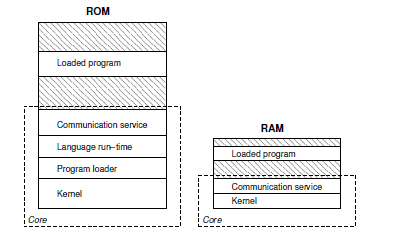
\includegraphics[width=0.9\textwidth]{Systemarchitektur_Contiki.png}
	\caption{Adam Dunkels, Bj\"orn Gr\"onvall, Thiemo Voigt: Contiki - a Lightweight and Flexible Operating System for Tiny Networked Sensors. \url{(Quelle:http://www.up.edu.ps/ocw/upinar/moodledata/872/moddata/assignment/970/1287/10.1.1.59.2303.pdf)}}
	\label{Systemarchitektur von Contiki}
\end{figure}
Der Core ist ein Basissystem und besteht aus dem Kernel, Bibliotheken, Ger\"{a}tetreiber und der Programm-Lader. Im allgemeinen sind \"Anderungen am Core nicht vorgesehen und nur unter Verwendung eines speziellen Bootloader m\"oglich. Die konkrete Aufteilung des Systems in Core und ladbare Programme wird beim Kompilieren des Systems entschieden und h\"angt von der Hardware-Plattform ab \cite[S. 7]{Walter:2010}. Ger\"atetreiber werden als Bibliotheken implementiert. 

\subsubsection{Events}
In Contiki kommunizieren Prozesse \"uber Events. Auch der Kernel versendet Events, um Prozesse \"uber ihren Status (Init, Continue, Exit) oder \"uber abgelaufene Timer zu Informieren. Zur Identifikation stehen dabei Event IDs zur Verf\"ugung. Die Event IDs 0-127 k\"onnen vom Benutzer frei vergeben werden, w\"ahrend die Prozess IDs ab 128 vom System genutzt werden. Grunds\"atzlich unterscheidet Contiki zwischen synchronen und asynchronen Events. 
\begin{itemize}
\item Asynchronen Events
\end{itemize}
Asynchrone Events sind eine Form der Deferred Procedure Call: asynchrone Events werden vom Kernel in einer Warteschlange gespeichert. Die Scheduling-Funktion des Kernels l\"auft nach Systemstart in einer Endlosschleife. In jedem Durchlauf wird ein Event aus der Schlange entnommen und wird einige Zeit sp\"ater an den Zielprozess weitergeleitet.
\begin{itemize}
\item Synchronen Events
\end{itemize}
Synchrone Events gleichen einem Funktionsaufruf. Die werden ohne Umweg \"uber die Warteschlange direkt an den Empf
\"anger-Prozess zugestellt \cite[S. 7]{Walter:2010}.  Mit der Funktion process\_post\_synch(\&example\_process, EVENT\_ID, msg) wird gezielt ein Prozess aufgerufen (ein Broadcast ist nicht m\"oglich). W\"ahrend der aufgerufene Prozess aktiv ist, blockiert der Aufrufer und setzt seine Ausf\"\"{u}hrung erst fort, wenn der aufgerufene Prozess die Kontrolle wieder abgibt.

\subsubsection{Prozesse}
Prozesse in Contiki implementieren ein Konzept namens Protothreads. Dies erlaubt es Prozessen, ohne den Overhead und die langen Prozesswechselzeiten von normalen Threads auszukommen. Gleichzeitig k\"onnen trotzdem andere Prozesse ausgef\"uhrt werden, falls ein Prozess auf ein Event (Timer, Nachricht von anderem Prozess...) warten muss. F\"ur die Entwicklung mit Prozessen ist wichtig, dass nicht-statische Variablen nicht zwischen zwei Aufraufen erhalten bleiben. Der relevante Status eines Prozesses sollte daher mithilfe von statischen Variablen abgelegt werden (siehe Variable i im folgenden Beispiel:

\begin{figure}[h!]
	\centering
		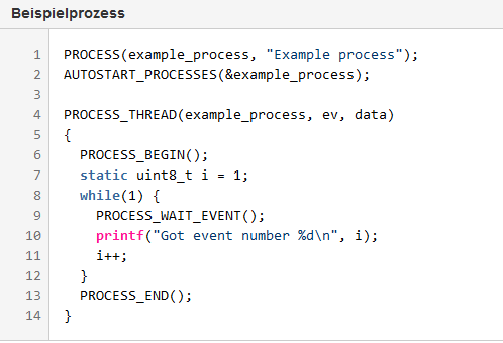
\includegraphics[width=0.9\textwidth]{Beispielprozess.png}
	\label{Beispielprozess}
\end{figure}
In Zeile 1 wird der Prozess initialisiert und in Zeile 2 automatisch beim Boot von Contiki gestartet. Zeile 4 beinhaltet die Deklaration. So k\"onnen andere Prozesse diesem Prozess Events (mit oder ohne Daten) schicken, auf die unser Beispielprozess mit ev und data zugreifen kann. Zeile 6 kennzeichnet den Beginn der tats\"achlichen Ablauflogik. Code \"uber dieser Zeile wird bei jedem Prozessaufruf ausgef\"uhrt, dies wird jedoch in den meisten F\"allen nicht ben\"otigt. Zeile 13 schlie{\ss}lich beendet den Prozess und entfernt ihn aus der Prozess-Liste des Kernels. In diesem Beispiel wird die Zeile jedoch nie erreicht, sodass er Prozess immer wieder aufgerufen wird, bis er von einem anderen Prozess beendet wird.
Wichtige Funktionen in Prozessen:
\begin{itemize}
\item PROCESS\_WAIT\_EVENT()- Wartet auf ein beliebiges Event, bevor die Ausf\"{u}hrung fortgesetzt wird
\item PROCESS\_WAIT\_EVENT\_UNTIL(condition) - Wartet auf ein beliebiges Event, setzt die Ausf\"{u}hrung aber nur fort, wenn die Bedingung erf\"{u}llt ist
\item PROCESS\_WAIT\_UNTIL() - Wartet, bis die Bedingung erf\"ullt ist. Muss den Prozess nicht zwangsl\"{a}ufig anhalten
\end{itemize}
Prozesse k\"onnen \"uber Events (siehe Events) oder Polling-Anfragen kommunizieren.  Polls sind Events mit hoher Priorit\"at und k\"onnen genutzt werden, um den angerufenen Prozess so schnell wie m\"oglich auszuf\"uhren. Sie
sind besonders bei der Abarbeitung von Hardware-Interrupts wichtig, da Interrupts-Handler keine Events, sondern nur
Polling-Anfragen absetzten d\"urfen \cite[S. 7]{Walter:2010}.
	
	
	% Bibliography
	\clearpage
	\clearscrheadfoot
	\ohead[Inhaltsverzeichnis]{Inhaltsverzeichnis}
	\chead[Uni Oldenburg]{Uni Oldenburg}
	\ihead[Malte Falk]{Malte Falk}
	\ofoot[Seminararbeit]{Seminararbeit}
	\cfoot[\pagemark]{\pagemark}
	\ifoot[WS 2013/14]{WS 2013/14}
	\ohead[Literaturverzeichnis]{Literaturverzeichnis}
	\printbibliography

\end{document}